\documentclass[11pt]{article}
\usepackage [french]{babel}
\usepackage [T1]{fontenc}

\usepackage[linesnumbered, ruled, french, onelanguage]{algorithm2e}
\usepackage{adjustbox}%Permet de centrer les figures dans la largeur de la page même si les figures sont plus larges que \textwidth
\usepackage{amssymb}
\usepackage{amsmath}
\usepackage[toc,page,title,titletoc,header]{appendix}
\usepackage{gensymb}%pour pouvoir écrire le signe °
\usepackage{geometry}%Pour changer la largeur des marges du document notamment
\usepackage{graphicx}
\usepackage{hyperref}%pour les liens dans la bibliographie
\usepackage{listings}
\usepackage{placeins}%pour utiliser FloatBarrier afin que les figure respectent bien leur position dans le code
\usepackage{slashbox}%Case séparée en deux tout en haut à gauche des tableaux à double entrées
\usepackage{stmaryrd}%pour les crochets à double barres d'intervalles de nombre entiers
\usepackage{tikz}
\usepackage{xcolor}%/definecolor et /color

\usepackage{etoolbox}%pour /AtBeginEnvironment
\AtBeginEnvironment{appendices}{\renewcommand{\thesection}{\Alph {section}}}%Pour recommencer à compter les sections à 0 en rentrant dans l'annexe et pour compter avec des lettres et non des chiffres
\renewcommand{\appendixpagename}{\centering Annexes}%Pour centrer le titre de la partie annexe
\renewcommand{\appendixtocname}{Table des annexes} % Pour faire apparaître les annexes dans la table of contents

%%%%%%%%%%%%%% Couleurs de: https://texblog.org/2011/06/11/latex-syntax-highlighting-examples/ %%%%%%%%%%%%%%
\definecolor{javared}{rgb}{0.6,0,0} % for strings
\definecolor{javagreen}{rgb}{0.25,0.5,0.35} % comments
\definecolor{javapurple}{rgb}{0.5,0,0.35} % keywords
\definecolor{javadocblue}{rgb}{0.25,0.35,0.75} % javadoc
 
\lstset
{
language=Java,
keywordstyle=\color{javapurple}\bfseries,
stringstyle=\color{javared},
commentstyle=\color{javagreen},
morecomment=[s][\color{javadocblue}]{/**}{*/},
numbers=left,
numberstyle=\tiny\color{black},
stepnumber=1,
numbersep=10pt,
tabsize=4,
showspaces=false,
showstringspaces=false}
%%%%%%%%%%%%%% Couleurs de: https://texblog.org/2011/06/11/latex-syntax-highlighting-examples/ %%%%%%%%%%%%%%





\author{}
\title{Ray-Tracer}
\date{}
\geometry{hmargin=3cm, vmargin=2cm}

\begin{document}
\tableofcontents
\newpage

\maketitle

\section{Détail des parties techniques}
\subsection{Le Ray Tracer}
\subsubsection{L'algorithme de base}
\label{rayTracingBase}
Les algorithmes de ray tracing permettent de générer des images fortes de réalisme grâce à la simulation de lois physiques appliquées à la lumière. Pour rendre une image par lancer de rayon, nous avons besoin de :
\begin{itemize}
	\item {Une caméra}
	\item {Une source de lumière}
	\item{Une scène contenant différents objets}
\end{itemize}
Le principe pour effectuer le rendu est ensuite assez simple. Nous lançons un rayon, partant de la caméra, à travers chaque pixel de l'image à rendre (on appelle cette image fictive par laquelle passent les rayons le "plan de la caméra"). Si ce rayon intersecte un objet de la scène, alors nous renvoyons la couleur de cet objet pour le pixel traversé par le rayon (voir annexe \ref{annexe:repreCamRayon}). Sinon, nous renvoyons la couleur du fond de la scène (ou de la skybox, section \ref{skybox}).
\subsubsection{L'ombrage de Phong}
\label{ombragePhong}

En appliquant le principe de la section \ref{rayTracingBase}, nous obtenons une image plate, sans aucun relief. Pour palier à cela, un modèle d'ombrage reste à implémenter. Ce sont en effet les ombres et les effets de lumière qui donnent aux images leur réalisme et leur profondeur. Un ombrage de Phong (imposé par le sujet) a donc été implémenté. L'ombrage de Phong consiste en l'addition de trois composantes distinctes:
\begin{itemize}
	\item {La composante ambiante. Elle permet de donner une luminosité minimale à la scène.}
	\item {La composante diffuse. Illumine d'autant plus l'objet que les rayons de lumière le frappe perpendiculairement.}
	\item {La composante spéculaire. Rend l'objet brillant en tenant compte de l'angle avec lequel les rayons de lumière rebondissent vers la caméra.}
\end{itemize}

\begin{figure}[h!]
	\adjustbox{center}{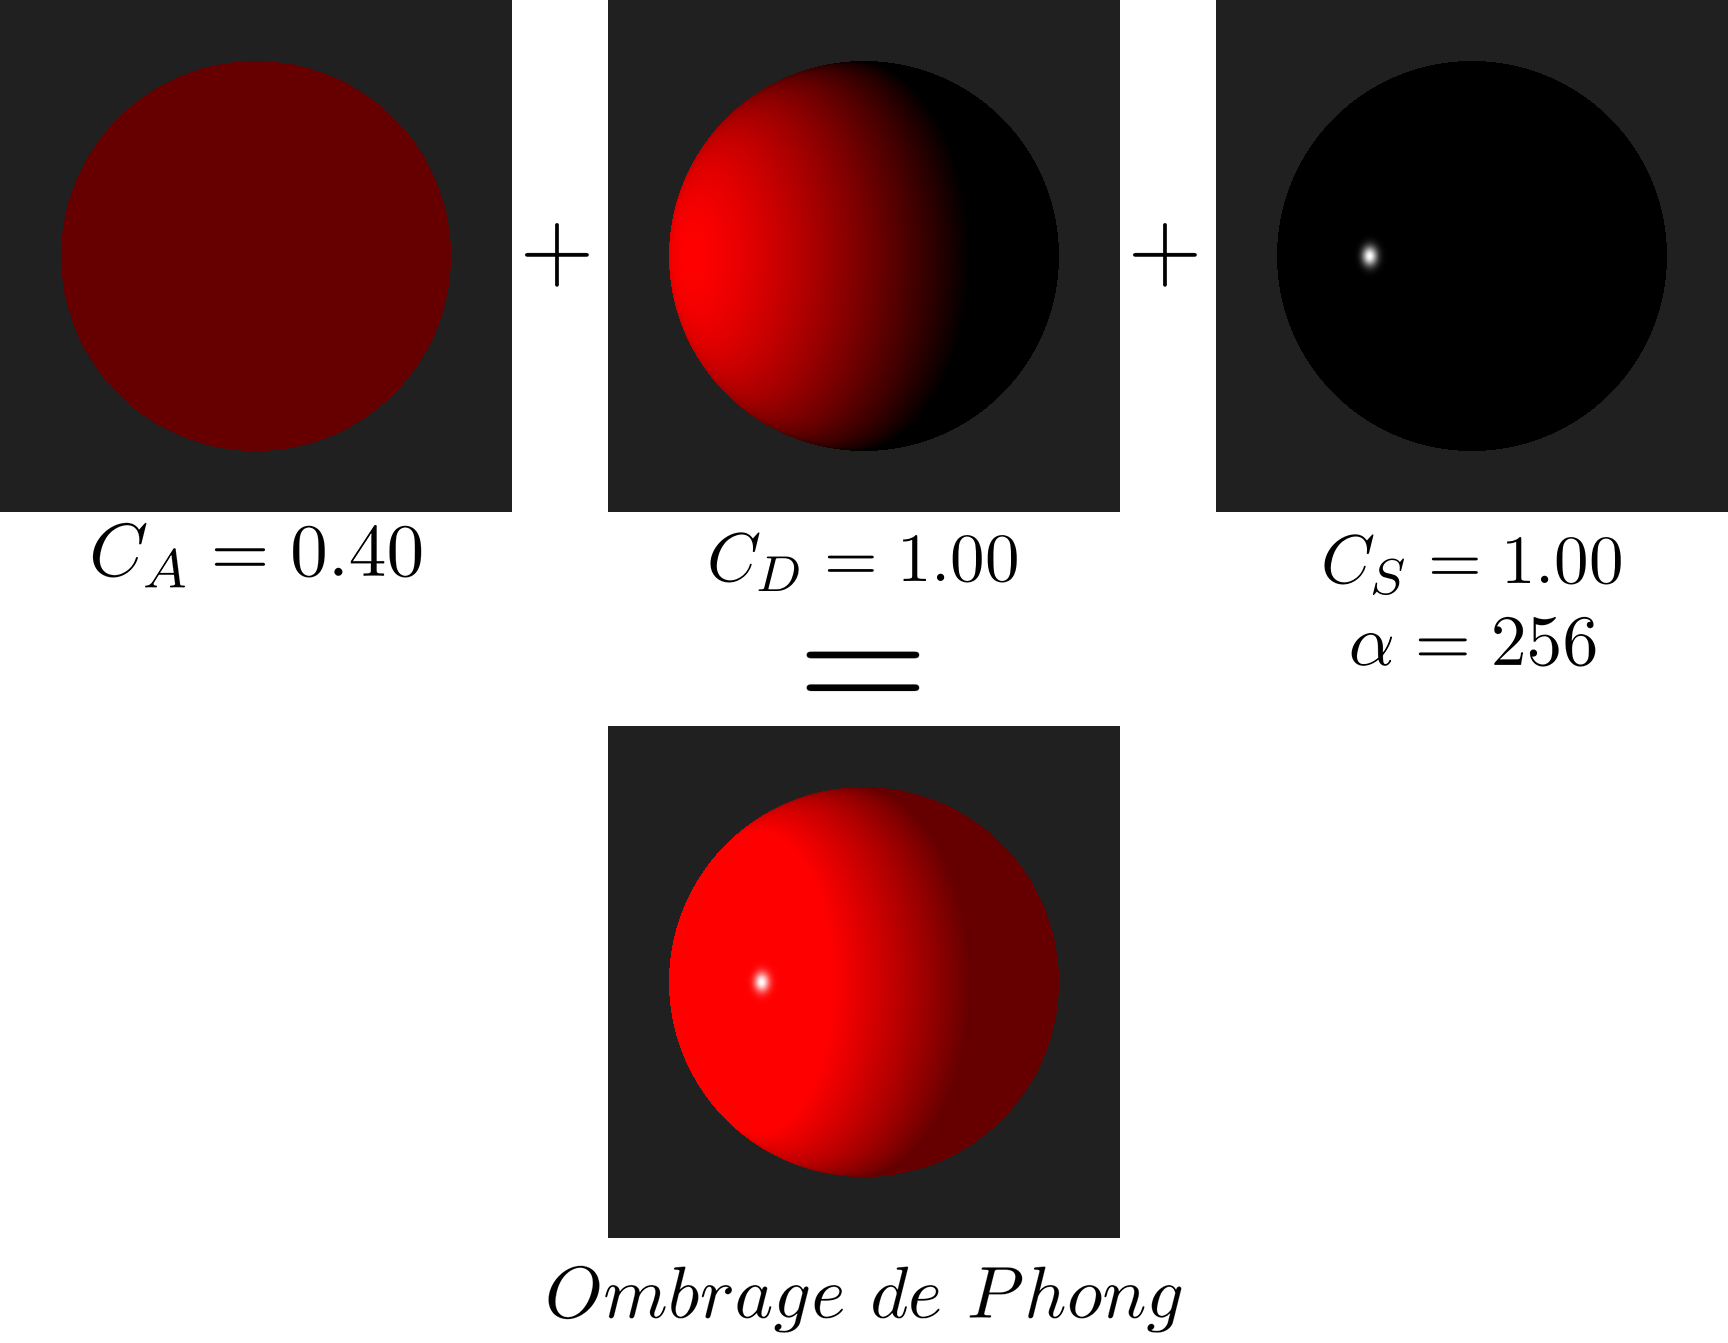
\includegraphics[width=0.75\textwidth]{img/rt/phongAddition.png}}

	\caption{Séparation des composantes de l'ombrage de Phong d'une sphère}
	\label{finalPhong}
\end{figure}
\FloatBarrier

\subsubsection{Les réflexions}
Une autre exigence du sujet (en plus de l'ombrage de Phong section \ref{ombragePhong}) était également l'implémentation de réflexions. Nous avons donc implémenté la réflexion des matériaux à la façon des miroirs. Autrement dit, nous supposons que les matériaux réflexifs de notre ray tracer sont parfaitement lisses et renvoient les rayons de lumière dans une seule et unique direction. Nous avons pour cela utilisé un algorithme récursif. En effet, si notre rayon frappe, un objet réfléchissant, il sera renvoyé dans une autre direction. De nouveau, si ce nouveau rayon réfléchi rencontre un autre objet réfléchissant, il sera une fois de plus renvoyé et ainsi de suite. Un algorithme récursif s'applique alors très bien ici.

\begin{algorithm}[H]
	\DontPrintSemicolon
	\KwIn{$\overrightarrow{R}$ le rayon incident (partant de la caméra)\\
					 $depth$ la profondeur actuelle de récursion}
	\KwOut{La couleur du pixel du plan de l'image par lequel est passé le rayon\\\hfill\\}

	\If(\tcp*[h]{La profondeur de récursion maximale a été atteinte}){depth == 0}
	{
		\Return{backgroundColor}
	}
	\hfill\\

	\If(\tcp*[h]{On vérifie si on a intersecté quelque chose}){$\overrightarrow{R}$.intersects(objetsScene)}
	{
		intersectedObject $\gets$ objet intersecté par $\overrightarrow{R}$\\\hfill\\

		\If(\tcp*[h]{Si l'objet intersecté est réfléchissant}){intersectedObject.isReflexive()}
		{
			$\overrightarrow{R_{reflect}} \gets$ computeReflectedDirection($\overrightarrow{R}$, $\overrightarrow{N}$)\\\hfill\\

			\Return{computeReflection($\overrightarrow{R_{reflect}}$, depth - 1)}{\tcp*[h]{On effectue un appel récursif pour relancer un rayon dans la direction du rayon réfléchi}}
		}
		\Else(\tcp*[h]{L'objet n'est pas réfléchissant, on va simplement retourner son ombrage de Phong})
		{
			\Return{phongShading()}
		}
	}
	\Else(\tcp*[h]{On a rien intersecté})
	{
		\Return{backgroundColor}
	}

	\caption{Algorithme de calcul des réflexions pour des objets non colorés - computeReflection}
	\label{algoReflections}
\end{algorithm}
\hfill\\
L'algorithme lance un rayon et vérifie si une intersection avec un objet a été trouvée ou non. Si oui, on s'assure que l'objet est réfléchissant. Dans ce cas, nous calculons la direction du rayon réfléchi et faisons un appel récursif à computeReflection. Nous avons également défini une profondeur maximale de récursion (ou nombre de réflexions maximal) afin d'éviter les récursions infinies (un rayon coincé dans une boîte dont les faces seraient toutes réfléchissantes par exemple). Si l'objet n'est pas réfléchissant, nous renvoyons simplement son ombrage de Phong comme vu dans la section \ref{ombragePhong}. Une représentation graphique de ce principe de réflexion est donné en annexe \ref{annexe:reflexionsRecursives}.\\
Avec une scène contenant des sphères réfléchissantes et d'autres mattes, nous obtenons le résultat suivant: 

\begin{figure}[h!]
	\adjustbox{center}{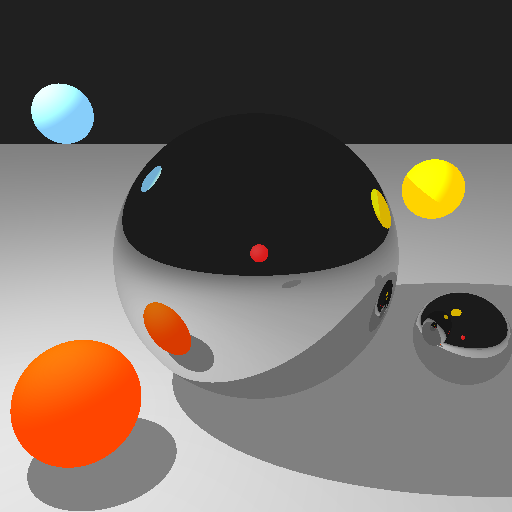
\includegraphics[width=0.5\textwidth]{img/rt/reflectionsDemo.png}}

	\caption{On peut voir une sphère rouge derrière la caméra grâce à la reflexion de la sphère centrale.}
	\label{reflectionsDemo}
\end{figure}
\FloatBarrier

\subsubsection{Les réfractions}
\label{refractions}

\subsubsection{Le damier et le ciel (skybox)}
Afin de rendre les réflexions de la scène plus remarquables et la scène moins monotone, nous avons implémenté un damier au sol au moyen d'UV mapping. Ainsi, pour chaque point d'intersection avec le plan représentant le sol, nous regardons si la somme des coordonnées X et Y du point d'intersection est paire ou non. Si la somme est paire, nous renverrons la première couleur du damier. Si elle est impaire, nous afficherons alors la deuxième couleur du damier.\\

\begin{figure}[h!]
	\adjustbox{center}
	{
		\begin{tikzpicture}[scale=1.5]
			%Dessin du damier
			\foreach \row in {0, 1, 2, ..., 4} 
			{
				\foreach \column in {0, 1, 2, ..., 4}
				{
					\pgfmathparse{Mod(\row + \column, 2) ? "white" : "black"}%On calcule le résultat de ligne + colonne modulo 2
					\colorlet{couleurDamier}{\pgfmathresult}%On transforme la chaîne de caractère donnée par pgfmathparse en couleur

					\fill[color=couleurDamier] (\row, \column) rectangle (\row+1, \column+1);%On colorie la case de la grille tikz
				}
			} 

			%Grille pour afficher les bordures
			\draw (0, 0) grid (5, 5);

			%Point de coordonnées
			%Dimensions de la grille
			\node (coin 0 0) at (-0.25, -0.25) {$(0, 0)$};
			\node (coin 5 5) at (5.25, 5.25) {$(5, 5)$};

			%Points exemple
			\filldraw[color=red] (1.3, 2.3) circle (4pt);
			\filldraw[color=red] (3.5, 3.5) circle (4pt);

			%Explications
			\node[draw, text width=3cm] (exp 1) at (-2-2.5cm, 2.3) {Somme des coordonnes (entières) impaire donc couleur blanche};
			\node[draw, text width=3cm] (exp 2) at (7, 3.5) {Somme des coordonnes (entières) paire donc couleur noire};

			\node (coords 1) at (1.3, -0.5) {$(x, y) = (1.3, 2.3)$};
			\node (coords 2) at (3.5, 5.5) {$(x, y) = (3.5, 3.5)$};

			%Lignes
			\draw[dashed, color=red, very thick] (exp 1)--(1.3, 2.3);
			\draw[dashed, color=red, very thick] (3.5, 3.5)--(exp 2);

			\draw[->, color=black!50!white, very thick] (1.3, 2.3)--(coords 1);
			\draw[->, color=black!50!white, very thick] (3.5, 3.5)--(coords 2);
		\end{tikzpicture}
	}
\end{figure}
\FloatBarrier

Bien que simple, cet algorithme d'UV mapping nous a permis d'embrayer sur l'implémentation d'une skybox. Notre skybox n'est autre qu'une image haute résolution d'un espace à ciel ouvert. Là encore, nous allons donc utiliser l'UV mapping. C'est en effet un moyen simple de convertir les coordonnées d'un point sur une sphère hypothétique de rayon 1 en des coordoonées 2D pour une image.

\subsection{Le multithreading}
\label{multithreading}
Les algorithmes de ray tracing sont réputés pour être lents à exécuter. Cependant, chaque pixel pouvant être calculé totalement indépendemment des autres, ces algorithmes sont des cibles parfaites pour la parallélisation de calcul. Nous avons donc mis en place, afin d'accélérer les temps de rendu, un multithreading de l'application grâce aux threads de Java. Pour ce faire, nous découpons l'image à rendre en plusieures "tuiles". Nous construisons ensuite une tâche à partir de chaque tuile. Une tâche consistant en:
\begin{itemize}
	\item{Un pixel de départ X et Y}	
	\item{Un pixel d'arrivée X et Y}
\end{itemize}
A partir de toutes ces tâches est ensuite construite une liste de tâche. Cette dernière servira aux threads lorsqu'ils viendront piocher dans la liste afin de récupérer les informations sur la zone de l'image qu'ils ont à rendre.
Un diagramme de classe illustre le fonctionnement du package multithreading dans la section \ref{packageMultithreading}.

\subsection{Les mouvements de caméra}
\label{mouvementsCamera}

Afin de pouvoir se déplacer dans la scène, nous nous sommes attelé à l'implémentation de mouvements de caméra grâce aux touches du clavier. Les mouvements possible sont: les translations de la caméra ainsi que les rotations de cette dernière autour des axes X et Y. Translater la caméra est assez simple. Il suffit de choisir un vecteur par lequel translater la caméra et appliquer cette même translation à l'origine des rayons (car leur origine doit rester la caméra) ainsi qu'à leur point de direction. Pour ce qui est des rotations, le principe est le même. En effet, faire une rotation de la caméra de 90\degree\ autour de l'axe Y revient à appliquer la même rotation aux points de direction des rayons. Afin de simplifier l'utilisation des translation et des rotations, nous avons utilisé une matrice appelée la CTWMatrix (Camera To World Matrix). Cette matrice rassemble les transformations de translation et de rotation appliquées à la caméra. Il n'y a donc plus qu'à multiplier le point que l'on veut transformer par cette matrice et le tour est joué.\\
Les matrices de rotation dans un espace de dimension 3 se présentent sous la forme suivante:

\begin{center}
	$R_{Y_{\alpha}} =
	\begin{pmatrix}
		cos(\alpha) & 0 & sin(\alpha)\\
		0 & 1 & 0\\
		-sin(\alpha) & 0 & cos(\alpha)
	\end{pmatrix}
	$ ;
	$R_{X_{\beta}} = 
	\begin{pmatrix}
		1 & 0 & 0\\
		0 & cos(\beta) & -sin(\beta)\\
		0 & sin(\beta) & cos(\beta)
	\end{pmatrix}
	$\\
	\textbf{Source: wikipedia} \cite{wikipediaRotationMatrices}
\end{center}
$R_{Y_{\alpha}}$ représente la matrice de rotation d'angle $\alpha$ autour de l'axe Y et $R_{X_{\beta}}$ son équivalent d'angle $\beta$ autour de l'axe X.

Une matrice de translation pour un vecteur $\overrightarrow{u}(a, b, c)$ se présente comme suit:
\begin{center}
	$T_{\overrightarrow{u}} =
	\begin{pmatrix}
		1 & 0 & 0\\
		0 & 1 & 0\\
		0 & 0 & 1\\
		a & b & c
	\end{pmatrix}
	$
\end{center}

On sait que la multiplication de deux matrices de rotation donne aussi une matrice de rotation combinant les deux rotations: $R_{Y_{\alpha}}$*$R_{X_{\beta}}$ = $R_{Y_{\alpha}X_{\beta}}$. On peut ensuite combiner la matrice de rotation obtenue avec notre de matrice de translation et on obtient:
\begin{center}
	$CTWMatrix =
	\begin{pmatrix}
		R_{YX_{0, 0}} & R_{YX_{0, 1}}  & R_{YX_{0, 2}}\\
		R_{YX_{1, 0}} & R_{YX_{1, 1}}  & R_{YX_{1, 2}}\\
		R_{YX_{2, 0}} & R_{YX_{2, 1}}  & R_{YX_{2, 2}}\\
		a & b & c
	\end{pmatrix}
	$
\end{center}

Multiplier un point par cette matrice revient alors à effectuer les rotations des deux matrices $R_{Y_{\alpha}}$ et $R_{X_{\beta}}$ et ensuite à translater le point résultant par le vecteur $\overrightarrow{u}(a, b, c)$.Tout cela en une seule opération de multiplication matricielle.

\section{Structuration du projet}
\subsection{Les packages}
\subsubsection{Liés au Ray Tracer}

Pour rendre une image, le RayTracer a besoin de:
\begin{itemize}
	\item{Une résolution de rendu}
	\item{Une scène contenant les objets à rendre}
	\item{Une ou plusieures sources de lumière}
	\item{Une caméra}
\end{itemize}
La résolution de rendu est fixe et est donnée au constructeur du RayTracer. La scène est les sources de lumière sont, quant à elles, dynamiques. La scène peut très bien être modifiée pendant le rendu et le RayTracer rendra les nouvelles images en conséquence. C'est pour cela que la scène est passée en argument de la méthode \textit{renderImage}. Il est alors facile de modifier la scène et d'ensuite la donner au RayTracer pour qu'il en fasse le rendu.

\begin{figure}[h!]
	\adjustbox{center}{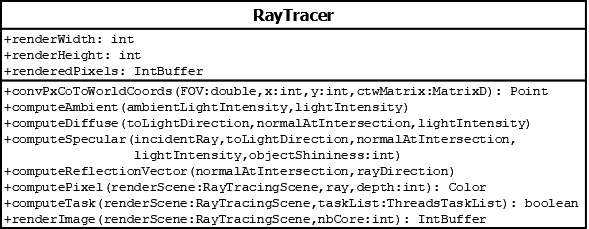
\includegraphics[width=\textwidth]{diagrammes/classe_RayTracer.png}}
	
	\caption{Diagramme de la classe RayTracer et de ses principales méthodes}
	\label{diagrammeRayTracer}
\end{figure}
\FloatBarrier

Les sources de lumière, la caméra et les objets de la scène dont a besoin le RayTracer sont des attributs de RayTracingScene. Comme énoncé plus haut, on peut ainsi facilement les modifier dynamiquement pendant le rendu.

\begin{figure}[h!]
	\adjustbox{center}{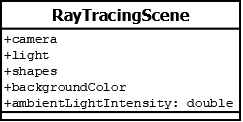
\includegraphics[width=0.42\textwidth]{diagrammes/classe_RayTracingScene.png}}
	
	\caption{Diagramme de la classe RayTracingScene}
	\label{diagrammeRayTracingScene}
\end{figure}
\FloatBarrier

La classe Camera, l'interface Light et la classe RayTracingScene s'organisent toutes dans le package scene:

\begin{figure}[h!]
	\adjustbox{center}{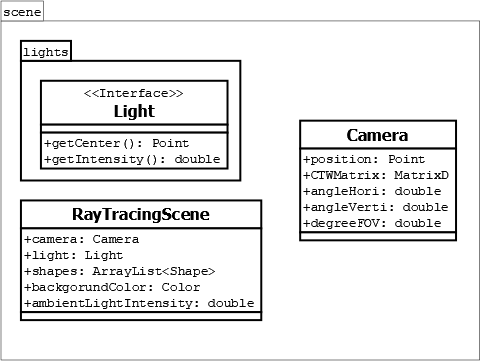
\includegraphics[width=0.75\textwidth]{diagrammes/package_scene.png}}
	
	\caption{Diagramme du package scene}
	\label{diagrammePackageScene}
\end{figure}
\FloatBarrier

\subsubsection{Le package materials}

Afin de colorer notre scène, nous devons donner une couleur aux formes des objets qui composent la scène. De plus, nous devons indiquer au RayTracer si l'objet est réflexif ou si au contraire il est mat, s'il est spéculaire et si oui à quel point, s'il est diffus...
Nous allons donc organiser toutes ces caractéristiques dans ce que l'on va appeler des matériaux.

\begin{figure}[h!]
	\adjustbox{center}{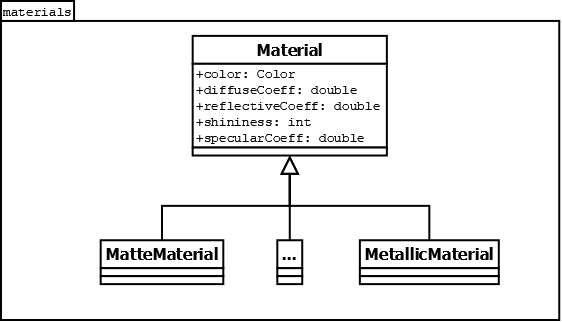
\includegraphics[width=0.75\textwidth]{diagrammes/package_materials.png}}
	
	\caption{Diagramme du package materials}
	\label{diagrammePackageMaterials}
\end{figure}
\FloatBarrier

Une classe mère Material permet de définir un matériau complètement arbitrairement. Toutes les caractéristiques peuvent être choisies comme on le souhaite.\\
Différentes classes héritent ensuite de cette classe mère afin de définir des catégories de matériau. Par exemple, MettalicMaterial va fixer la réflectivité du matériau à un certain point, de même pour sa diffusion, sa spécularité etc... Toutes ces caractéristiques fixées d'une certaine façon donnera donc au matériau un aspect métallique. Il ne restera plus qu'à donner un MetallicMaterial à un objet de la scène pour qu'il ait un aspect métallique pendant le rendu. Le visuel des matériaux peut donc être personnalisé assez facilement et intuitivement avec l'utilisation des matériaux.

\section{Mesures de performance}
Comme présenté dans la section \ref{multithreading}, nous application tire partie de toute la puissnce du processeur de la machine. Le but étant de réduire le temps de calcul, nous présentons dans cette section les gains perçus en terme de performances.\\
Nous comparerons les temps de rendu par image pour différentes résolutions et différents nombre de threads. L'image sera toujours découpée en $nbThread^2$ tuiles.

\begin{figure}[h!]
	\adjustbox{center}{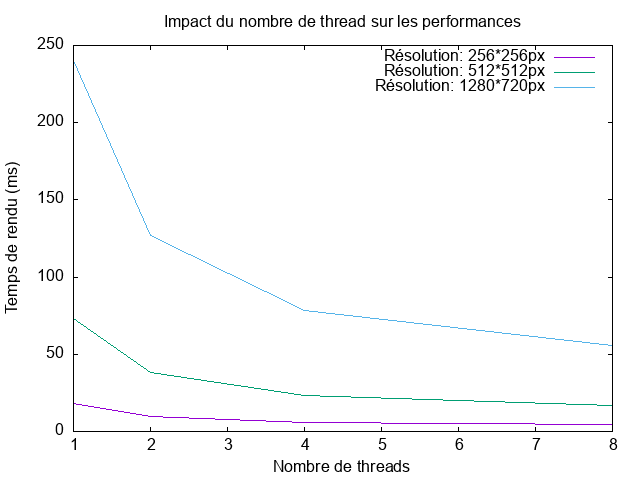
\includegraphics[width=1\textwidth]{img/rt/MultithreadingGraph.png}}
	
	\caption{Graphe de l'impact du nombre de thread sur le temps de rendu par image}
	\label{graphMultithreading}
\end{figure}
\FloatBarrier
Toutes les mesures ont été faites sur un CPU disposant de 8 processeurs. La scène rendue est la même que celle de la \figurename\ \ref{reflectionsDemo}.\\
On observe une réduction significative des temps de rendu quand le nombre de threads utilisé augmente. On passe en effet, pour une résolution de 512*512, de 72.87ms en moyenne à 16.72ms de temps de calcul par image. Cela se traduit par un affichage fluide d'un peu moins de 15 images par seconde avec 1 thread. Avec 8 threads, nous passons à environ 60 images par seconde. Les performances ont donc été multipliées par 4.\\
Cette multiplication des performances nous permet entre autre de pouvoir profiter de mouvements fluides lorsque l'on déplace la caméra. Sans ces 8 threads, les mouvement seraient saccadés et peu agréables dû aux temps de rendu trop importants. Bien entendu, les temps de rendu dépendent aussi de la complexité de la scène. Nous avons remarqué que les matériaux réfractifs ont tendance à être plus lourds à calculer que les matériaux mats. Cela s'explique par le fait qu'un matériau réfractif demande de nombreux appels récursifs.






\newpage%Nouvelle page pour les annexes
\begin{appendices}
	\section{Le ray tracer}
		\begin{figure}[h!]
			\adjustbox{center}{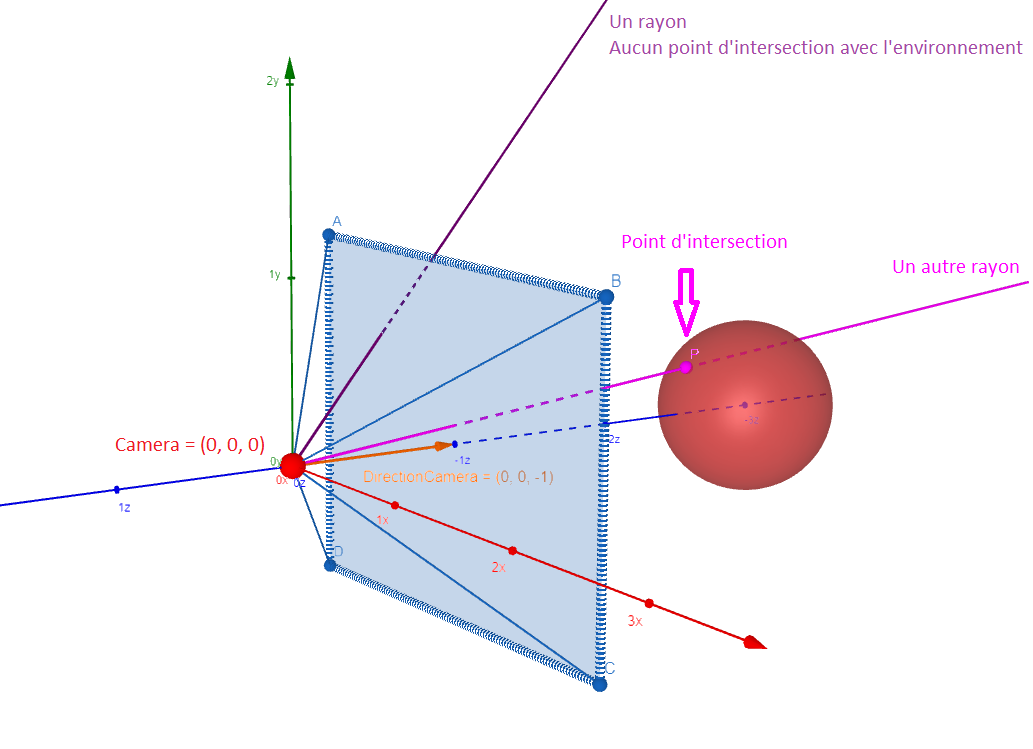
\includegraphics[width=1.1\textwidth]{img/rt/repCam2Rayonsv2.png}}
		
			\caption{Des rayons sont tirés depuis la caméra dans sa direction de regard. Nous cherchons les points d'intersection avec les objets de la scène}
		\end{figure}
		\FloatBarrier
		\label{annexe:repreCamRayon}

		\begin{figure}[!h]
			\adjustbox{center}{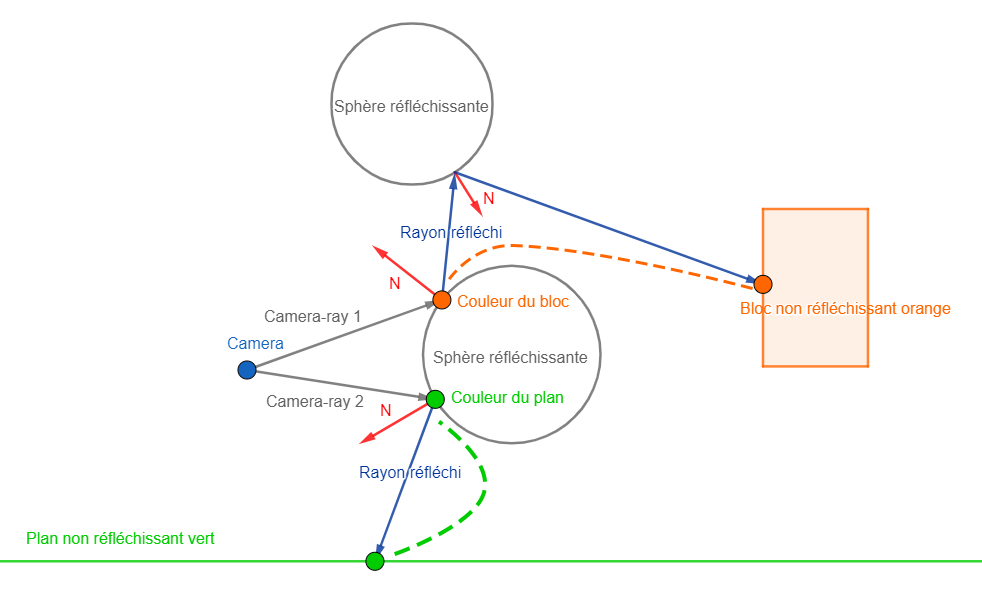
\includegraphics[width=1.1\textwidth]{img/rt/reflectionsSchema.png}}
		
			\caption{Exemple de rebonds successifs des rayons jusqu'à un objet non réfléchissant}
			\label{reflectionsSchema}
		\end{figure}
		\FloatBarrier
		\label{annexe:reflexionsRecursives}
\FloatBarrier
\end{appendices}

\newpage%Nouvelle page pour la bibliographie
\nocite{*}
\bibliographystyle{unsrt}
\bibliography{bibliography/sources}

\end{document}